\documentclass[]{article}

\usepackage{amsfonts}
\usepackage{amsmath}
\usepackage{graphicx}
\usepackage{amsthm}
\usepackage{svg}
\usepackage{enumitem}
\usepackage{color}
\usepackage{float}


\graphicspath{{images/}}
\setsvg{svgpath={./images/}}

\newtheorem{thm}{Theorem}[subsection]
\newtheorem{Def}{Definition}[subsection]
\newtheorem*{thm*}{Theorem}
\newtheorem*{def*}{Definition}
\newtheorem{lem}{Lemma}[subsection]

\newcommand{\compav}[1]{\textbf{\textcolor{blue}{#1}}}
\newcommand{\compat}[1]{\textbf{\textcolor{red}{#1}}}
\newcommand{\shiftleft}[2]{\makebox[0pt][r]{\makebox[#1][l]{#2}}}
\newcommand{\tilda}{\big{\char"7E}}



%opening
\title{Geodesic Flow on the Necker Cube Surface}
\date{}
\author{Pavel Javornik}

\begin{document}


\maketitle



\begin{center}

\includesvg[width=4.8in]{cubecoverphoto}\\
\end{center}

\begin{abstract}
This paper classifies the periodic and drift-periodic trajectories on the Necker cube surface, a periodic surface built out of squares popular in optical illusions.
\end{abstract}



\newpage
\section{Introduction}

The purpose of the following paper is to study the geodesic flow on the periodic surface depicted above, which is formed from an infinite collection of unit squares. We call this surface the Necker cube surface after Louis Albert Necker's ``Necker Cube$_{1}$,'' which became a popular optical illusion. M.C. Escher's adaptation of the cube in Metamorphosis I$_{2}$ briefly features the Necker cube surface (See Figure $\ref{fig:Escher}$).The term Necker Cube is used interchangeably to refer to Escher's surface adaptation and Necker's optical illusion. For the purposes of the following paper, we will be using either Necker Cube or $\mathbf{S}$ to refer to the periodic cube tiling that appears in Escher's work.


\begin{figure}[H]
\begin{center}
\includegraphics[scale=0.5]{escher.jpg}
\caption{The Necker cube as it appears briefly in Metamorphosis I}
\label{fig:Escher}
\end{center}
\end{figure}

The initial (rational) trajectories of any given flow fall into only one of two categories.
\compat{The definitions below seem redundant. Perhaps you want ${\mathcal O}$ and ${\mathcal E}$}

\begin{def*}
Let $v$ be a vector of the form $(x,y)\in\mathbb{Z}^{2}$. We call $v$ an \textbf{odd-odd} vector if x and y are relatively prime and both odd. We denote the \textbf{set of all odd-odd vectors} by $\mathcal{O}$. We say that $v$ is an  \textbf{even-odd} vector if x and y are relatively prime, and x is even if and only if y is odd. We denote the \textbf{set of all even-odd vectors} by $\mathcal{E}$.
\end{def*}

We consider every (rational) initial trajectory on the surface to fall into one of the two categories, otherwise it is a positive scalar multiple of some direction. Given some initial point $x_{0}$ on the surface embedded in real space and some vector direction in real space, $\bar{v}$, our initial trajectory,$v$, is taken as an isomorphism from the planar subspace of $\mathbb{R}^{3}$ that contains $\bar{v}$. The three possible cases are the auxiliary planes, $x=0, y=0, z=0$, whose projections onto $\mathbb{R}^{2}$ are given by $(0,y,z)\mapsto(-z,y)$, $(x,0,z)\mapsto(x,-z)$, and $(x,y,0)\mapsto(x,y)$ respectively and relative to the standard bases of $\mathbb{R}^{3}$. We take $-z$ to be positive, and consider vectors that lie outside of these subspaces as degenerate cases. From there we prove the following:

\begin{thm*}{Given an initial trajectory, $\theta\in\mathbb{R}^{2}$, and geodesic path, $\gamma$, on $\mathbf{S}$ with initial trajectory $\theta$, the following is true:} \compat{There is no flow in a fixed direction because when trajectories move to new squares they may be traveling different directions.}
\compav{Can I use gamma as a path on S?}
\begin{enumerate}[label=(\roman*)]
\item If $\theta$ belongs to $\mathcal{O}$, then $\gamma$ is closed on $\mathbf{S}$ and homeomorphic to $\mathbb{R}/\mathbb{Z}$.
\item If $\theta$ belongs to $\mathcal{E}$, then $\gamma$ is drift-periodic on $\mathbf{S}$.

\end{enumerate}
\end{thm*}

\compav{Archiving for later:\\If $\theta$ is of the form (x,y) such that x or y are irrational, then $\phi^{\theta}_{t}$ is uniquely ergodic on $\mathbf{S}$. \compat{We should move the discussion of ergodicity outside the theorem.}	}

\compav{Stopped here. Continued in Section 2.}

The Necker Cube is a member of the family of infinite Euclidean cone surfaces built out of rectangles with vertices of cone angle $3\pi$ and $\frac{3\pi}{2}$. We wish to study the surface in the case where we glue only squares with edges of length 1. Specifically, we want to study geodesic flows on this surface and to prove that properties of the initial trajectory angle determine whether or not the geodesic will close or drift periodically. 

The determining factor is simply whether or not the trajectory angle vector direction $(a,b)$, relative to the bottom and left edges of any square face, has integer values $a$,$b$ (where $a$ and $b$ are relatively prime) are of the same parity (odd-odd slope) or different parities (even-odd slope). We choose to neglect cases where paths are incident with vertices, and proceed to treat them as singularities. With these conditions in place we found that any geodesic with an initial odd-odd trajectory closes on the surface, while the even-odd cases drift periodically, tending to infinity. We aim to prove the following:



\subsection{Discussion of Proof}
\subsection{Related work}


To better understand this surface, we will adapt methods used in the study of Veech surfaces to suit our needs. These methods have become incredibly valuable to anyone studying rational billiard flows on a variety of compact or (in the case of infinite surfaces) non-compact surfaces. Geodesic flows in these problems are characterized as point masses moving along frictionless surfaces that experience perfectly elastic collisions with the boundaries of the surface. The straight line path is then deformed by a reflection over the boundary in the opposite direction. Translation surfaces constructed in the following manner therefore take on symmetric properties in accordance to these transformations and the types of boundaries the point mass might encounter. That is to say that orienting these flows requires that the translation surface itself be reflected to realign the flow. These translation surfaces are often described as being "unfolded" by some billiard flow, or strung along a laundry line of polygons congruent to the base. In the later sections we will describe how our surface's canonical form deforms geodesic flows by rotation and how we can use these rotations and edge-crossings to determine whether or not a geodesic will close.

What inspired this paper was the work done by Hubert et al. [Hu] on the Ehrenfest-Wind Tree model. Any readers who are familiar with their paper or the Tree model will most likely notice the similarities between the quotient spaces of the two surfaces and the properties that determine whether or not geodesic paths close. While similar, these surfaces are not entirely identical. The effect that a boundary collision has on a geodesic alters the dynamical properties of the surface. Or perhaps they better demonstrate properties of the surface itself. Another fundamental difference between the two is that the Necker Cube is a surface with cone angles surrounding an infinite number of singularities on the surface. The problem has to take into careful consideration what it means for a path to cross a saddle connection between these singularities of the translation surface.



\subsection{Procedure}
The Necker Cube surface has an interesting construction process that lets us take each face of the cube and arrange them in any way we choose so long as we do not change how the edges are identified, or glued together. It is preferable to study the flows on this surface as though every cube has been flattened onto the plane. This means that we can consider the cube step to be tiled by infinitely many of L-shaped surfaces whose edges are identified by rotation.

Doing so greatly reduces the number of possible directions that a flow might travel. Since every edge of this L-shaped surface is identified to another either by translation or a 90 degree rotation, any straight line path on this flattened version of the Necker Cube can experience only one of four possible directions at any given time, whereas the Necker Cube would've had considerably more.

Moreover, every face of this L-shaped surface is given by rotating its associated face on the Necker Cube about the x or y axis, affine translations, or a combination of the two. By cutting and gluing every half-cube of the Necker Cube in a consistent fashion, we can preserve the areas of the faces and distances between any two points on the surface with the flattening procedure. We describe this procedure as piecewise maps that are comprised of compositions of Euclidean matrices and translations of points relative to the L-shape onto a subset of $\mathbb{R}^{2}$ with square shaped holes cut out. Since rotations and translations of points preserves distance between them, the path lengths and  associated properties of geodesic flows remain invariant.

The image of this map is a flattened version of the Necker Cube. (See FIG [MATLAB MODEL]). From that surface we construct a new one made out of four copies of original, each rotated by some factor of 90 degrees so as to realign the geodesic flows and assure that they can only travel in one possible direction. This four-fold surface is then a cover of the original surface. We consider every possible direction to be a "phase" of the flow, and index the planes accordingly. Any edges in the holes of the surface are identified with an edge on an adjacent phase plane (By rotation of $\pm \frac{\pi}{4}$). Any point on this surface has a coordinate in $\mathbb{R}\times\mathbb{R}\times\mathbb{Z}_{4} $

Similarly, we take the quotient space of the flattened Necker Cube centered around each square shaped hole and realign its flows by rotation. The resulting surface is a compact branch cover of the quotient space. Singularities on the translation surface have a total angle that is some multiple of $2\pi$. We consider the translation surface to be a base surface of the four-fold cover, and study its properties to prove our main theorem. In particular, we wish to determine what effect a member of the translation surface's Veech group has on both the surface and geodesic flow in hopes that it would shine some light on odd-odd even-odd phenomenon.



 $SL_{2}(\mathbb{R})$

\section{Constructing the Surface \& Isometric Variant}
\compav{Started up here again 6/21/17}

This section will detail how the Necker cube (See Figure \ref{fig:cubexyz}) is constructed out of an infinite set of unit squares, and explain the process by which we flatten the structure in such a way that preserves distances, and makes it simpler for us to describe the behavior of the geodesic flows that come into contact with these edges.

\begin{figure}[H]
\begin{center}
\includesvg[width=3in]{cubesxyz}
\caption{The Necker cube embedded in space.}
\label{fig:cubexyz}
\end{center}
\end{figure}

\subsection{The Necker Cube Surface}

To build the surface out of infinitely many unit squares, we take the union of the instances of three squares, each lying on planes orthogonal to the other two and sharing an edge with exactly one other square. The three squares have only one vertex in common.

First we divide the planes $x,y,z=k$ for some integer $k$ in such a way that they are composed entirely out of unit squares. We want to index each of these squares by integer triples and some label A,B, or C. i.e. squares on planes of the form $z=k$ will have an A label, $x=k$ a B label, and $y=k$ a C label. Let $m,n,p\in\mathbb{Z}$. Then each square based at $(m,n,p)$ is defined as follows:

\vspace{0.2in}
\begin{tabular}{p{10cm}c}
\begin{align*}
\mathbf{A}_{m,n,p} = [m, m+1]\times[n,n+1]\times\{p\}, 
\\\mathbf{B}_{m,n,p} = \{m+1\}\times[n,n+1]\times[p-1,p],
\\\mathbf{C}_{m,n,p}= [m,m+1]\times\{n+1\}\times[p-1,p].
\end{align*}
&
\shiftleft{0.8in}{\raisebox{-1in}{
\includegraphics[scale=1]{label.png}}}
\end{tabular}
\vspace{0.2in}\\
\noindent For the sake of convenience, B and C are shifted in order to associate each integer triple that satisfies the linear condition $m+n+p=0$ with an instance of the cube that $\mathbf{S}$ is composed of. Furthermore, we  separate $\mathbf{S}$ into the sets:
\begin{align*}
\mathbf{A}=\bigcup\big{\{}\mathbf{A}_{m,n,p}: m+n+p=0\big{\}},
\\\mathbf{B}=\bigcup\big{\{}\mathbf{B}_{m,n,p}: m+n+p=0\big{\}},
\\\mathbf{C}=\bigcup\big{\{}\mathbf{C}_{m,n,p}: m+n+p=0\big{\}}.
\end{align*}

\noindent We can now give a formal definition of the Necker Cube.

\begin{Def} The \textbf{Necker Cube}, denoted by $\mathbf{S}$, is the surface made up of unions of unit squares of the form $\mathbf{S} = \mathbf{A}\cup\mathbf{B}\cup\mathbf{C}$.\end{Def}

\noindent $\mathbf{S}$ is the surface portrayed in Figure \ref{fig:cubexyz}. 

\subsection{The Flattened Form}
We will show that $\mathbf S$ is isometric to a a topological quotient of a particular subset of the plane. We call this quotient $\mathbf{U}$, and the subset of the plane $\mathbf P$ (See Figure $\ref{fig:uprimeu}$).
The subset $\mathbf P$ is the region of the plane with unit squares removed:
\begin{equation}
\label{eq:P}
\mathbf{P} = \mathbb{R}^{2}\text{ }\backslash\bigcup_{m,n \in {\mathbb Z}} \big{\{}(u,v):u\in(2m-\frac{1}{2},2m+\frac{1}{2}),\text{ } v\in(2n-\frac{1}{2},2n+\frac{1}{2})\big{\}}.
\end{equation}

\compat{Illustrating refering to equations: Recall $\mathbf{P}$ was defined in \eqref{eq:P}.}


\begin{figure}[H]
\begin{center}
\includesvg[width=1.5in]{uprime}
\end{center}
\caption{The subset $\mathbf P$ of the plane with unit squares removed at every even integer pair.} \compat{Perhaps just use one.}
\label{fig:uprimeu}
\end{figure}

\noindent On $\mathbf P$ we define a relation $\sim$ that identifies the sides of the boundaries of each hole in pairs. Each side is identified with another side of the same hole by rotation about the bottom left or top right corners of the hole by $\pm\frac{\pi}{2}$. The result is an edge identification as seen here (centered at each even coordinate pair): \compat{I think overall this is very good and completely defines the relation. You may want to tweak it to make it even more clear. You expressed some concerns about the vertices.}

\begin{figure}[H]\centering
\includesvg[width=2in.]{quotient}
\end{figure}
\noindent We call this relation $\mathbf{R}$. \compat{How about $\sim$?} What $\mathbf{R}$ essentially does is translates every hole to the origin and identifies the edges by reflecting over the line $y=x$. If these points coincide, then they are indeed the same point on the boundary. Otherwise, every point that is not on the boundary belongs to its own class. We can safely assume this wont identify edges improperly, since we translate every boundary so as to situate the unit holes over the origin. For example, if we took two edges that do not belong to the same hole then by that same translation and reflection the two edges couldn't possible coincide.  \compat{This paragraph doesn't seem to add much.}

\begin{Def}
content...
\end{Def}

\begin{Def}{$\mathbf U$}\\
$\mathbf U$ is equal to the quotient space $\mathbf{P}/\mathbf{R}\times\{0\}$
\end{Def}

\compav{Stopped here. 6/21/17}

\compat{I would use as an introductory paragraph: ``We will show that $\mathbf S$ is isometric to a topological quotient of a subset of the plane.''}

Before describing the transformation that takes $\mathbf{S}$ to its flattened form, it would be best to define the relations on a subset of the plane that preserves the identification of edges. We will call this surface $\mathbf{U}'$. However, the flattening of the surface takes $\mathbf{S}$ to a translation of $\mathbf{U}'$, we call $\mathbf{U}$ (See $\ref{fig:uprimeu}$). We will denote the metric preserving map from $\mathbf{S}$ to $\mathbf{U}$, by $\Psi$. Defining these edge identifying relations over $\mathbf{U}'$ is more convenient for us than defining them over $\mathbf{U}$, but defining $\Psi$ is more convenient when the map is taken to $\mathbf{U}$ due to the nature of the construction of $\mathbf{S}$. \compat{I found this paragraph awkward. I would just go ahead and define the region in the plane.}



Now we will describe exactly how to construct $\mathbf{U}'$. Take the subset of the real plane, 
$$,$$ 
\compat{I would write $(m-\frac{1}{2},m+\frac{1}{2}) \times (n-\frac{1}{2},n+\frac{1}{2})$.}
with open unit squares cut out at every even integer pair and let $\mathbf{U}'$ represent the flattened structure with the proper edge identifications with the first "hole" centered at the origin. We will describe this surface as a cross product of the auxiliary plane, $z=0$ and the image of the natural map from $\mathbf{P}$ to its quotient space with the following relation on $\mathbf{P}$:

\begin{gather*}
\text{Let } x_{0}=(u_{0},v_{0}),x_{1}=(u_{1},v_{1}) \in \mathbf{P}. \text{Let } \mathbf{R} \text { be a relation given, } x_{0}\mathbf{R}x_{1} \\ \text{ iff } x_{0}=x_{1}
 \text{ or if }x_{0},x_{1} \in {\partial} \left( \left[2m-\frac{1}{2},2m+\frac{1}{2}\right] \times \left[2n-\frac{1}{2},2n+\frac{1}{2}\right] \right)\\
  \left[\begin{array}{c}
u_{1} -2m
\\v_{1}-2n
\end{array}\right] = \left[\begin{matrix}
0 && 1\\
1 && 0
\end{matrix}\right]
\left[ \begin{array}{c}u_{0}-2m\\
v_{0}-2n
\end{array}\right]
\\\text{For some }m,n\in\mathbb{Z}. \end{gather*}

The relation will either identify every point to itself or, in the case where any two points lie on the boundary of the square shaped holes, take the center of each square hole in the plane to the origin and reflect it over the line $y=x$ to match up these points accordingly.  Let $N: \mathbf{P} \rightarrow \mathbf{P}/\mathbf{R}$ denote the natural map from every point on $\mathbf{P}$ to its appropriate equivalence class. Now, let $\mathbf{U}' = Im N \text{ }\times\{0\}$ be the flat representation of the surface that has been translated so as to center the first square cut-out region over the origin. The map $\mathbf{U}\rightarrow\mathbf{U}'$ is given by an affine translation of the surface $(x,y,z) \mapsto (x-\frac{3}{2},y-\frac{3}{2},z)$. (The point at the origin of $\mathbf{S}$ is mapped to $(-\frac{3}{2},-\frac{3}{2},0) \text{ on } \mathbf{U}'$).

\compav{Stopped here. Continued in Sec. 3.}

\newpage
\subsection{Flattening $\mathbf{S}$}
This section will describe the isomorphic map $\Psi:\mathbf{C}\rightarrow\mathbf{U}$, its inverse, $\Psi^{-1}:\mathbf{U}\rightarrow\mathbf{C}$, and prove that $\mathbf{C}$ and $\mathbf{U}$ are isometric.

The flattening procedure can be represented as a series of cuts made along edges parallel to the z-axis. The gluing structure is preserved by the relations defined on $\textbf{U}$ and $\textbf{U}'$. 

\begin{center}
\includesvg[width=2.3in]{cubesxyzcut}
\raisebox{0.4in}{\includesvg[width=2.3in]{u}}
\text{The images of } $\Psi^{-1}(\mathbf{U})$ (left)\text{ and }$\Psi(\mathbf{S})$ (right)
\end{center}

$\Psi$ is defined piecewise, and denote each subset of $\mathbf{C}$ with the letters $A$, $B$, $C$. We do the same for $\mathbf{U}$ but use instead $A'$, $B'$, $C'$. 

\begin{gather*}
	\text{Let }x,y,z\in\mathbb{R}. \text{ Then}
	\\A=\bigcup\big\{\mathbf{C}\cap\{(x,y,p)\in\mathbb{R}\}: p\in\mathbb{Z}\big\}
	\\B=\bigcup\big\{\mathbf{C}\cap\{(x,n,z)\in\mathbb{R}\}: n\in\mathbb{Z}\big\}
	\\C=\bigcup\big\{\mathbf{C}\cap\{(m,y,z)\in\mathbb{R}\}: m\in\mathbb{Z}\big\}
	\\\text{are the collection of the faces of cubes that lie on planes that are parallel to one another.}
	\\\text{As shown here:}
\end{gather*}



To describe the subsets $A'$, $B'$, and $C'$ properly we will introduce the function $\mu_{n}:\mathbb{R}\rightarrow \left[0,n\right) $ as shorthand for the family of functions that take a real number to its residue class of reals modulo n, for some integer n.

\begin{gather*}
	\text{Let }u,v\in\mathbb{R}. \text{Then }
	\\A'= \{(u,v,0): 0<\mu_{2}(u)\leq 1 ,\hspace{4mm} 0<\mu_{2}(v)\leq 1\}
	\\B'= \{(u,v,0): 1<\mu_{2}(u)\leq 2,\hspace{4mm} 0<\mu_{2}(v)\leq 1\}
	\\C'= \{(u,v,0): 0<\mu_{2}(u)\leq 1,\hspace{4mm} 1<\mu_{2}(v)\leq 2\}
	\\\text{are the collections of the associated faces of the flattened structure.}
\end{gather*}



Now we will define $\Psi$ piecewise.

\begin{equation}
\Psi\left[\begin{array}{c}
	x\\y\\z
\end{array}\right] 
= 
\begin{cases}
	\left[ \hspace{2mm} \begin{matrix}
		1 & 0 & 0 \\
		0 & 1 & 0 \\
		0 & 0 & 1
	\end{matrix}\hspace{3mm}\right]

	\left[\begin{array}{c}
	x - \left\lfloor x \right\rfloor
	\\ y- \left\lfloor y \right\rfloor
	\\ -(z - \left\lfloor z \right\rfloor)
	\end{array} \right]
	+
	\left[\begin{array}{c}
		2 \left\lfloor x \right\rfloor
		\\ 2\left\lfloor y \right\rfloor
		\\ z - \left\lfloor z \right\rfloor
	\end{array} \right]
		& \text{if } (x,y,z)\in A	\vspace{2mm}
	\\
		
		
	\left[ \begin{matrix}
	0 & 0 & 1 \\
	0 & 1 & 0 \\
	-1 & 0 & 0
	\end{matrix}\hspace{2mm}\right]
	\left[\begin{array}{c}
		x - \left\lfloor x \right\rfloor
		\\ y- \left\lfloor y \right\rfloor
		\\ -(z - \left\lfloor z \right\rfloor)
		\end{array} \right]
	+
		\left[\begin{array}{c}
			2 \left\lfloor x \right\rfloor
			\\ 2\left\lfloor y \right\rfloor
			\\ x - \left\lfloor x \right\rfloor
		\end{array} \right]
			& \text{if } (x,y,z)\in B	\vspace{2mm}
	\\
	
		\left[ \begin{matrix}
		1 & 0 & 0 \\
		0 & 0 & 1 \\
		0 & -1 & 0
		\end{matrix}\hspace{2mm}\right]
		\left[\begin{array}{c}
			x - \left\lfloor x \right\rfloor
			\\ y- \left\lfloor y \right\rfloor
			\\ -(z - \left\lfloor z \right\rfloor)
			\end{array} \right]
		+
			\left[\begin{array}{c}
				2 \left\lfloor x \right\rfloor
				\\ 2\left\lfloor y \right\rfloor
				\\ y - \left\lfloor y \right\rfloor
			\end{array} \right]
				& \text{if } (x,y,z)\in C	\vspace{2mm}
\end{cases}
\end{equation}

We chose to preserve the matrix structure in order to emphasize the manner in which every square is taken to $\mathbf{U}$ from $\mathbf{C}$ and vice-versa. The negations of some of these variables are a result of this structure being built so as the integer triples lie on the plane $z=-(x+y)$. Defining the maps this way also makes it possible to generalize it for any surface constructed in a similar manner of taking unions of three faces of rectangular prisms in real space. (i.e. $\chi_{m,n,p}$ belongs to a larger family of rectangular arrangements parameterized by the dimensions of the rectangular prism. In this case, $\chi_{m,n,p}$ is a member of this family whose dimensions are $1\times1\times1$). 

Now we will define the inverse map, $\Psi^{-1}$, in a similar manner. 

\begin{equation}
	\Psi^{-1}\left[\begin{array}{c}
		x\\y\\z
	\end{array}\right] 
	= 
	\begin{cases}
		\left[ \hspace{2mm} \begin{matrix}
			1 & 0 & 0 \\
			0 & 1 & 0 \\
			0 & 0 & 1
		\end{matrix}\hspace{3mm}\right]
	
		\left[\begin{array}{c}
		x - 2\left\lfloor \frac{x}{2} \right\rfloor
		\\ y- 2\left\lfloor \frac{y}{2} \right\rfloor
		\\ z
		\end{array} \right]
		+
		\left[\begin{array}{c}
			\left\lfloor \frac{x}{2} \right\rfloor
			\\ \left\lfloor \frac{y}{2} \right\rfloor
			\\ -(\left\lfloor \frac{x}{2} \right\rfloor + \left\lfloor \frac{y}{2} \right\rfloor )
		\end{array} \right]
			& \text{if } (x,y,z)\in A'	\vspace{2mm}
		\\
		\left[ \hspace{2mm} \begin{matrix}
			0 & 0 & -1 \\
			0 & 1 & 0 \\
			1 & 0 & 0
		\end{matrix}\hspace{0mm}\right]
	
		\left[\begin{array}{c}
		-(x - 2\left\lfloor \frac{x}{2} \right\rfloor)
		\\ y- 2\left\lfloor \frac{y}{2} \right\rfloor
		\\ z
		\end{array} \right]
		+
		\left[\begin{array}{c}
			1+\left\lfloor \frac{x}{2} \right\rfloor
			\\ \left\lfloor \frac{y}{2} \right\rfloor
			\\ -(\left\lfloor \frac{x}{2} \right\rfloor + \left\lfloor \frac{y}{2} \right\rfloor -1)
		\end{array} \right]
			& \text{if } (x,y,z)\in B'	\vspace{2mm}

	\\
	
		\left[ \hspace{2mm} \begin{matrix}
			1 & 0 & 0 \\
			0 & 0 & -1 \\
			0 & 1 & 0
		\end{matrix}\hspace{0mm}\right]
	
		\left[\begin{array}{c}
		x - 2\left\lfloor \frac{x}{2} \right\rfloor
		\\ -(y- 2\left\lfloor \frac{y}{2} \right\rfloor)
		\\ z
		\end{array} \right]
		+
		\left[\begin{array}{c}
			\left\lfloor \frac{x}{2} \right\rfloor
			\\1+ \left\lfloor \frac{y}{2} \right\rfloor
			\\ -(\left\lfloor \frac{x}{2} \right\rfloor + \left\lfloor \frac{y}{2} \right\rfloor -1)
		\end{array} \right]
			& \text{if } (x,y,z)\in B'	\vspace{2mm}
			
	\end{cases}
\end{equation}

By using properties of the floor function, one can show that $\Psi$ is indeed a bijective, invertible map. All that is left to show is that $\Psi$ preserves distance.

\begin{thm}{$\mathbf{C}$ and $\mathbf{U}$ are isometric.}\\
Proof. Let $(\mathbf{C}, d)$ and $(\mathbf{U}, d')$ be topological spaces with their respective metrics. Let $a,b\in\mathbf{C}$, and let $\Psi(a)=a',\Psi(b)=b'\in\mathbf{U}$. We will denote the distance between $a$ and $b$ by $D=d(a,b)$, and the distance between $a'$ and $b'$ by $D'=d'(a',b')$. Since $\Psi$ and $\Psi^{-1}$ are linear transformations that act on subsets of auxiliary planes in $\mathbb{R}^{3}$, the images of any curves on $\mathbf{C}$ or $\mathbf{U}$ under these maps will not be deformed and retain their lengths. Thus, $D \leq d'(\Psi(a), \Psi(b)) = d'(a',b') = D'$. Likewise, $D' \leq d(\Psi^{-1}(a'),\Psi^{-1}(b')) = d(a,b) = D$. Therefore $D=D'$, and $\Psi$ and $\Psi^{-1}$ are metric preserving maps between $\mathbf{C}$ and $\mathbf{U}$. $\qed$
\end{thm}

As a consequence of this theorem, any dynamical properties of geodesic flow on the surface $\mathbf{U}'$ immediately applies to $\mathbf{C}$. ($\mathbf{U}'$ and $\mathbf{U}$ are trivially isometric).

\subsection{Comparing Geodesic Behavior on Both Surfaces}
Two immediate observations that can be made in regards to geodesic flows on the surface was that any trajectory with slope one closes, and any flows with horizontal or vertical trajectories drift. Observe the path behavior of three different flows on the surface:



The figure above shows us some very simple paths on the surfaces. We use the three vectors, (0,1), (1,0), and (1,1), as a sort of basis for proving our theorem. Included in the appendix are a few more simulated flows of various trajectories. We've color coded the trajectories in the image above for path c to represent one of four phases

\newpage
\section{The Four-Fold Cover and Translation Surface}
\compav{Started here again.}
The following section is concerned with defining a quotient of $\mathbf{U}'$ (see Figure $\ref{fig:quotient}$), and using that space to construct a translation surface. In addition we will describe a cover made from four copies of $\mathbf{U}'$ that aligns geodesic flow and behaves as a cover of our translation surface. \compat{Revisit to make sure it summarizes the section}


\subsection{Four-Fold Cover of $\mathbf{U}$}
A geodesic on $\mathbf{U}$ viewed as a sequence of line segments on $\mathbf{P}$ travels in at most four directions which differ by a rotation of a multiple of $\frac{\pi}{2}$. This is a consequence of the edge identifications taking the boundary of a hole on $\mathbf{P}$ to its counterpart by a rotation of ninety degrees. To each of these directions we associate an element of $\mathbb{Z}/4\mathbb{Z}$ to signify one of the four possible directions of the geodesic flow at any given time. Given that, we can create a four-fold cover of $\mathbf{U}$ as a topological quotient of $\mathbf{P}\times\mathbb{Z}/4\mathbb{Z}$. For every integer pair centered around every hole of $\mathbf{P}\times\mathbb{Z}/4\mathbb{Z}$, create the edge identifications that takes one plane to the next in the following manner:

\begin{figure}[H]
\centering
\includesvg[width=4in]{utilda}
\label{fig:utilda0}
\caption{$\tilde{\mathbf{U}}_0$ is a branched cover of $\mathbf{U}$ of degree four.}
\end{figure}

$\tilde{\mathbf{U}}_0$ has the obvious covering map that takes every point on $\tilde{\mathbf{U}}_0$ and projects it onto $\mathbf{U}$. We define the edge identifications as a relation on $\mathbf{P}\times\mathbb{Z}/4\mathbb{Z}$. For $i\in[-\frac{1}{2},\frac{1}{2}]$:



\begin{equation}
\begin{split}
(2m+i, 2n-\frac{1}{2};j)\sim(2m-\frac{1}{2},2n+i;j+1)\\
(2m+i, 2n+\frac{1}{2};j)\sim(2m+\frac{1}{2},2n+i;j+1)\\
\vspace{0.2in}\text{for } (m,n;j) \in \mathbb{Z}^{2}\times\mathbb{Z}/4\mathbb{Z}.
\label{eq:rel2}
\end{split}
\end{equation}

We define $\tilde{\mathbf{U}}_0$ to be the topological quotient, $(\mathbf{P}\times\mathbb{Z}/4\mathbb{Z})/\sim$. $\tilde{\mathbf{U}}_0$ is a Euclidean cone surface with four vertices at each hole centered at $(2m,2n;\mathbb{Z}/4\mathbb{Z})$ of cone angle $6\pi$.

\subsection{Symmetries of $\tilde{\mathbf{U}}_0$}
There are certain translational and rotational symmetries of $\mathbf{P}\times\mathbb{Z}/4\mathbb{Z}$ that we use to define isometries. These isometries are well-defined and induce isometries on $\tilde{\mathbf{U}}_0$ that respect the edge identifications we made earlier.

\begin{Def}Let $m,n\in\mathbb{Z}$. The {family of translation maps}, $\mathbf{T}^{m,n}_{0}$ on $\mathbf{P}\times\mathbb{Z}/4\mathbb{Z}$, is given as $\mathbf{T}^{m,n}_{0}(u,v;j)=(u+2m,v+2n;j)$.\newline
The {family of ``rotational" isometries} on $\mathbf{P}\times\mathbb{Z}/4\mathbb{Z}$ is given as the automorphism $\mathbf{R}_0(u,v;j)=(u,v;j+1)$, where $\mathbf{R}_0$ is an action on $\mathbf{P}\times\mathbb{Z}/4\mathbb{Z}$ of order 4.
\end{Def}

\begin{lem}$\mathbf{T}^{m,n}_{0}$ induces a well-defined isometry on $\tilde{\mathbf{U}}_0$.
\begin{proof}
It suffices to show that $\mathbf{T}^{m,n}_{0}$ preserves the edge identifications $\eqref{eq:rel2}$. Let $x,y\in\mathbf{P}\times\mathbb{Z}/4\mathbb{Z}$, where $x=(u_x,v_x;j_x)$ and $y=(u_y,v_y,j_y)$. Clearly, if $x=y$, then $\mathbf{T}^{m,n}_{0}(x)=\mathbf{T}^{m,n}_{0}(y)$. Hence, $T_0$ is bijective. Consider the case where $x\neq y$. Let $x\sim y$ and observe that if $x,y$ lie on any of the edges, then $\mathbf{T}^{m,n}_{0}(x)=(u_x+2m,v_x+2n;j_x)$ and $\mathbf{T}^{m,n}_{0}(y)=(u_y+2m,v_y+2n;j_y)$ for $m,n\in\mathbb{Z}$. Since $x\sim y$, either $j_y=j_x+1$, or $j_x=j_y+1$. Suppose the former is true. Then for $i$ in the interval $[-\frac{1}{2},\frac{1}{2}]$:

\begin{equation*}
\begin{split}
(2m_x+2m+i, 2n_x+2n-\frac{1}{2};j_x)\sim(2m_x+2m-\frac{1}{2},2n_x+2n+i;j_y)\\\text{ and }\hspace{2in}\\
(2m_x+2m+i, 2n_x+2n+\frac{1}{2};j_x)\sim(2m_x+2m+\frac{1}{2},2n_x+2n+i;j_y),\\
\end{split}
\end{equation*}
which is the result of $T_0$ acting on the edges, and $m_x,n_x$ are integers that originally ensured that $x\sim y$. Since $m,n$ are arbitrarily chosen integers, $T_0$ maps one edge to exactly one other as the edges surrounding each hole are indexed by a unique pair of even integers and $T_0$  is a bijective map that respects that construction. A similar argument holds for the case where $j_x=j_y+1$. Therefore, $\mathbf{T}^{m,n}_{0}(x)\sim\mathbf{T}^{m,n}_{0}(y)$.
\end{proof}
\end{lem}

We will call the induced isometry on $\tilde{\mathbf{U}}_0$, $\bar{\mathbf{T}}^{m,n}$.

\begin{thm}$\mathbf{R}_{0}$ induces an isometry on $\tilde{\mathbf{U}}_0$
\begin{proof}
\compav{might rethink including $R_0$}.
\end{proof}
\end{thm}

\subsection{Four-fold Translation Cover}

 Now we will show that $\tilde{\mathbf{U}}_0$ is isometric to a translation surface via another induced isometry on $\mathbf{P}\times\mathbb{Z}/4\mathbb{Z}$. We would like this map to rotate each individual plane of $\mathbf{P}\times\mathbb{Z}/4\mathbb{Z}$ about the origin in such a way that edges one the boundaries are identified strictly by translation. Every plane that is represented as an element of $\mathbb{Z}/4\mathbb{Z}$ is conveniently acted on by a ninety degree rotation matrix, whose power we take to be that very same element.


We express $\phi:\mathbf{P}\times\mathbb{Z}/4\mathbb{Z} \rightarrow \mathbf{P}\times\mathbb{Z}/4\mathbb{Z}$ as $\phi(u,v;j) = (u',v';j)$, where

\begin{equation}
	\left[\begin{array}{c}
		u'\\v'
	\end{array}\right] =
		\left[ \hspace{1mm} \begin{matrix}
				0 & 1\\
				-1 & 0
			\end{matrix}\hspace{1mm}\right]^{j}\left[\begin{array}{c}
					u\\v
				\end{array}\right].
\label{eq:phi}
\end{equation}
This is clearly an isometry, as rotations preserve distance and $j\mapsto j$.

\begin{Def} Let $\sim$ be the equivalence relation $\eqref{eq:rel2}$, and $\phi$ be the isometric map on $\mathbf{P}\times\mathbb{Z}/4\mathbb{Z}$ $\eqref{eq:phi}$. Define a new relation obtained from $\sim$ as $x_1\sim_{\phi}x_2$ iff $\phi^{-1}(x_1) \sim \phi^{-1}(x_2)$ for $x_1,x_2\in\mathbf{P}\times\mathbb{Z}/4\mathbb{Z}$. A new surface is obtained as the topological quotient $\tilde{\mathbf{U}}=$ $(\mathbf{P}\times\mathbb{Z}/4\mathbb{Z})/\sim_{\phi}$.\label{eq:simphi}
\end{Def}


\begin{figure}[H]
\centering
\includesvg[width=3.65in]{utildaprime}
\caption{$\tilde{\mathbf{U}}$ with edges identified, and holes indexed relative to $\mathbf{P}\times\{0\}$.}
\label{fig:utilda}
\end{figure}


\begin{thm}{The following statements are true:}
\begin{enumerate}[label=(\roman*)]
\item The map $\phi$ induces a well-defined isometry from $\tilde{\mathbf{U}}_0$ to $\tilde{\mathbf{U}}$.
\item $\tilde{\mathbf{U}}$ is a translation surface.
\end{enumerate}
\begin{proof}
It will again suffice to show that $\phi$ preserves $\tilde{\mathbf{U}}_0$'s edge identifications to prove $(i)$. Let $x_1,x_2\in\mathbf{P}\times\mathbb{Z}/4\mathbb{Z}$. From $\tilde{\mathbf{U}}$'s definition $\eqref{eq:simphi}$, we see that $x_1\sim_{\phi} x_2$ if and only if $\phi^{-1}(x_1) \sim \phi^{-1}(x_2)$. By taking $\phi^{-1}(x_1)$ and $ \phi^{-1}(x_2)$ to be the pre-images of the quotient map onto $\tilde{\mathbf{U}}_0$, it is clear that $\phi$ preserves identifications. Otherwise, it would contradict the definition. Furthermore, since $\phi$ is a well-defined isometry, there is an induced isometry on the topological quotients, $\tilde{\mathbf{U}}_0$ and $\tilde{\mathbf{U}}$.\newline
Let $x_1\sim_{\phi} x_2$. Then $\phi^{-1}(x_1) \sim \phi^{-1}(x_2)$. Let $\phi^{-1}(x_1)=(u_1,v_1;j_1)$ and $\phi^{-1}(x_2)=(u_2,v_2;j_2)$. Without loss of generality, suppose that $j_2=j_1+1$. Let $i$ vary over the interval $[-\frac{1}{2},\frac{1}{2}]$, and $m,n$ be integers such that they satisfy the relation $\phi^{-1}(x_1) \sim \phi^{-1}(x_2)$. If $\phi$ acts on these these two points, then $x_1 = (u_1',v_1';j_1)$ and $x_2 = (u_2',v_2';j_1+1)$. But we know that $(u_1',v_1')=M^{j_1}(u_1,v_1)$ and $M^{j_1+1}(u_2',v_2')=(u_2,v_2)$, where $M$ is the rotation matrix as in $\phi$. Thus, $M^{j_1}(u_1,v_1)\times\{j_1\}\sim_\phi M^{j_1+1}(u_2,v_2)\times\{j_1+1\}$. By multiplying through by $M^{-j_1}$ prior to taking the cross-product, we obtain $(u_1,v_1)\times\{j_1\}\sim_\phi M(u_2,v_2)\times\{j_1+1\}$. Since $M(u_2,v_2) = (v_2,-u_2)$, we can express the relation $\sim_\phi$ as
\begin{equation*}
\begin{split}
(2m+i, 2n-\frac{1}{2};j_1)\sim_\phi(2n+i, -(2m-\frac{1}{2});j_1+1),\\
\text{ and }\hspace{1.2in}\\
(2m+i, 2n+\frac{1}{2};j_1)\sim_\phi(2n+i, -(2m+\frac{1}{2});j_1+1).\\
\end{split}
\end{equation*}
It is clear from this relation and figure $\ref{fig:utilda}$ that $\tilde{\mathbf{U}}$ is a translation surface.
\end{proof}
\end{thm}
We will denote this induced isometry as $\bar{\phi}$.

%A geodesic on this translation surface can be realized as a sequence of edge crossings on the phase planes. By taking a quotient of this surface, a closed straight-line path can be lifted from the quotient onto $\tilde{\mathbf{U}}$, and then projected onto $\mathbf{U}$ to study geodesic behavior of any given direction.

\subsection{Constructing $\tilde{\mathbf{U}}$'s base surface}
In this section we use the induced isometries on $\tilde{\mathbf{U}}_0$, and the map $\bar{\phi}:\tilde{\mathbf{U}}_0\rightarrow\tilde{\mathbf{U}}$ to define a set of rotational and translational symmetries of $\tilde{\mathbf{U}}$ such that its quotient over the action of these maps are faithful representations of $\tilde{\mathbf{U}}_0$ in terms of how the holes in $\mathbf{P}\times\mathbb{Z}/4\mathbb{Z}$ are indexed. It is briefly mention after the definition of $\tilde{\mathbf{U}}$ that $\bar{\phi}$ alters this scheme relative to $\tilde{\mathbf{U}}_0$. 

\begin{Def}We call the {family of $\tilde{\mathbf{U}}$'s translational symmetries} $\mathbf{T}^{m,n}$ and define it to be the composition of the induced isometric maps: $\mathbf{T}^{m,n}$ = $\bar{\phi}\circ\bar{\mathbf{T}}^{m,n}\circ\bar{\phi}^{-1}$.
\end{Def}

We can see that $\mathbf{T}^{m,n}$ is indeed an isometry on $\tilde{\mathbf{U}}$ as it is composed of the induced isometries, $\bar{\phi}$ and $\bar{\mathbf{T}}^{m,n}$ . We can take the quotient of the translation surface $\tilde{\mathbf{U}}$ over the action of $\mathbf{T}^{m,n}$ to obtain a base surface that realizes $\tilde{\mathbf{U}}$ as an infinite $\mathbb{Z}^2$ cover.

\begin{Def}
The translation surface $\mathbf{M}$ is given as the quotient  $\tilde{\mathbf{U}}/\mathbf{T}^{m,n}$.
\end{Def} 

\begin{figure}[H]
\centering
\includesvg[width=4in]{mtilda}
\caption{The surface $\mathbf{M}$ with labeled vertices and identified edges. Labels I, II, III, and IV identify the individual planes indexed by \{0,1,2,3\}, respectively.}
\label{fig:mtilda}
\end{figure}

The new surface, $\mathbf M$, is a genus 5 translation surface with the surjective quotient map $f:\tilde{\mathbf{U}}\rightarrow\mathbf M$ that sends every point of $\tilde{\mathbf{U}}$ to its modular equivalent. $\mathbf M$ is a Euclidean cone surface with four singularites of cone angle $6\pi$ on the corners of the square cut out from each of the squares labeled I,II,III, and IV. Those squares have their opposite edges identified by translation. $\mathbf M$ might be thought of as a collection of four $2\times2$ square tori with a unit square cut out from their centers, and identifications made on these edges so as to associate one torus with exactly two others. Although a single edge only relates two of the tori, the vertices in the centers are the same throughout $\mathbf M$.
\newpage

\subsection{$\mathbf M$ as a Veech Surface}
By a series of cutting and gluing operations, $\mathbf M$ has this symmetric representation as a square-tiled staircase (Figure $\ref{fig:staircase}$). The vertices of cone angle $2\pi$ can be found on the centers of the squares in the figure below where the black lines intersect. 
\begin{figure}[H]
\centering
\includesvg[width=4in]{mtildastaircase}
\caption{$\mathbf{M}$ as a square-tiled staircase with cone singularities identified.}
\label{fig:staircase}
\end{figure}
As a result of Gutkin-Judge [citation], $\mathbf M$ is a Veech surface whose Veech group is commensurable to $SL(2,\mathbb Z)$. In order to determine which elements of orientation preserving automorphisms, denoted Aut$^{+}(\mathbf M)$, have derivatives that belong to the Veech group of $\mathbf M$, SL($\mathbf M$), it is necessary to study $\mathbf M$'s various symmetries and cylinder decompositions.

The derivatives of these automorphisms form the affine group, Aff$^+(\mathbf M)$. One such group contained in Aff$^+(\mathbf M)$ is SO$(2,\mathbb{Z})$, the group generated by rotations of order 4. Even though the other elements in $\mathbb{D}_4$ are derivatives of automorphisms of $\mathbf M$, we will only consider those of determinant +1.

Observe from the following image that $\mathbf M$ has a uniform cylinder decomposition in both the horizontal and vertical directions:

\begin{figure}[H]
\centering
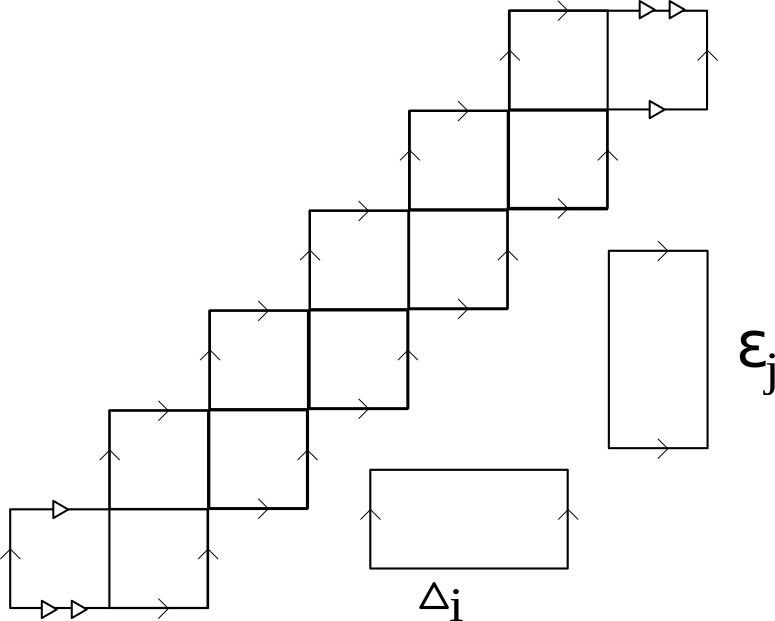
\includegraphics[width=4in]{cylinderdecomp.pdf}
\caption{Horizontal and Verical Cylinders overlayed.}
\label{fig:decomp}
\end{figure}

Both sets of cylinders are indexed $0\leq i, j \leq 5$. Every cylinder is composed of two unit squares with edges identified by translation. We start counting the cylinders from the bottom-most cylinder and increment the index as the cylinders fill the surface going "up" the staircase. $\small{\mathcal{E}}_0$ is the first cylinder at the bottom whose identifications are \em{not} \normalfont the solid triangles. $\small{\mathcal{E}}_5$ is the cylinder whose edges are paired by the solid triangles. $\Delta_{i}$ has the more standard representation starting from the bottom-most horizontal cylinder. 

We define the \emph{inverse modulus} of a cylinder to be the ratio of a cylinders circumference to its width, $\mu^{-1}=\frac{c}{h}$. A \emph{Dehn-twist} of a cylinder is an automorphism of the cylinder of the form  $(x,y)\mapsto(x,y+\mu^{-1} x \mod{h})$, where $x$ and $y$ are points on the cylinder relative to its circumference and height respectively. According to [need to cite something], a translation surface whose finite cylinder decompositions in orthogonal directions form a set of inverse moduli. The lowest (rational) common multiple of the set of all these values match up to give global affine diffeomorphisms of the surface, whose matrix representations are 
\begin{equation*}
\left[ \hspace{1mm} \begin{matrix}
				1 & \pm \lambda\\
				0 & 1
			\end{matrix}\hspace{1mm}\right] \text{ and }
			\left[ \hspace{1mm} \begin{matrix}
							1 & 0\\
							\pm \lambda & 1
						\end{matrix}\hspace{1mm}\right],
\end{equation*}
where $\lambda$ is the lowest common multiple.

Fortunately, the cylinders $\Delta_{i}$ and $\small{\mathcal{E}}_j$, as i and j vary, all have the same inverse moduli. Therefore, $\lambda=$ l.c.m.($\mu^{-1}_{\Delta_i}\cup\mu^{-1}_{\mathcal{E}_j}$) $=2$.

\begin{figure}[H]
\centering
\includesvg[width=2.6in]{cylinderskew}
\caption{Stabilizing Dehn-twists of the horizontal/vertical cylinders}
\label{fig:skew}
\end{figure}

Consequently, 
\begin{equation}
\left< \left[ \hspace{1mm} \begin{matrix}
				1 &  2\\
				0 & 1
			\end{matrix}\hspace{1mm}\right] \text{ , }
			\left[ \hspace{1mm} \begin{matrix}
							1 & 0\\
							 2 & 1
						\end{matrix}\hspace{1mm}\right] \right>
						\subset \text{SL}(\mathbf M).
\end{equation}
This group is also known as the \emph{Sanov Subgroup}, a free group of rank 2. We take the group generated by ninety degree rotations and these two elements to be the group $\mathbb{X}\subset \text{SL}(\mathbf M)$.
\newpage
\subsection{$\mathbb X$'s Action on $\mathbf M$'s Homology}
The group $\mathbb X$ consists of the set of all derivatives of Aut$^+(\mathbf M)$, whose action on the absolute homology of $\mathbf{M}$ extends to an action on the homology of $\mathbf{M}$'s $\mathbb{Z}^2$-cover, $\tilde{\mathbf{U}}$. $\mathbf{M}$'s cylinder decomposition gives way to a set of homology classes that serve as a basis for $H_1(\mathbf{M},\mathbb Z)$. For a total of 12 cylinders, there are 12 curves:

\begin{figure}[H]
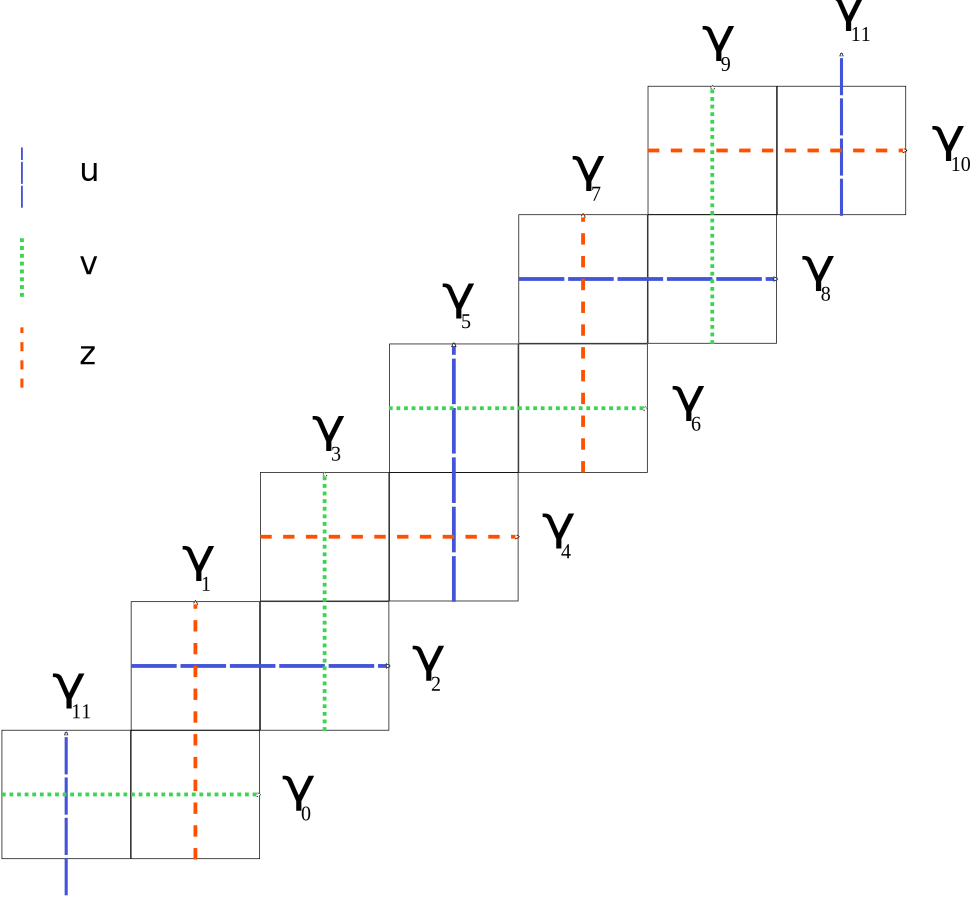
\includegraphics[width=3in]{homologyclass.png}
\centering
\end{figure}
Every curve intersects two others. By constructing a $12\times12$ matrix where the rows represent each curve and the columns represent their intersections with other curves, we can see that the rank of said matrix is 10. This is to be expected as the genus of $\mathbf M$ is 5. From these curves we construct homology classes $u,v,$ and $z$. $u$ and $v$ are the curves that were the outermost edges of the tori in $\mathbf{M}$'s original representation (Figure $\ref{fig:mtilda}$). We can see from Figure $\ref{fig:utilda}$ that crossing over one of these edges corresponds to a shift of the even integer index pair that determines exactly which of the quotients of $\tilde{\mathbf{U}}$ a terminal point of a lifted path on the surface belongs to. That point is identified with the triple $(m,n,\mathbb Z/4\mathbb{Z})$, with integers $m,n$. The $z$ class of cylinder curves lie on the cylinders that take a path from one plane to the next in our cover. Since one plane is related to exactly two others, it is impossible to go directly from the first to the third or the second to the fourth, and vice versa. 

Regardless, $u$ and $v$ are the most important homology classes that we use to determine whether or not a lifted path properly closes on the four-fold cover.  Let $\alpha:[0,1]\rightarrow\mathbf M$ be a curve on the surface such that $\alpha(0)=\alpha(1)=x_0\in\mathbf{M}$. Take $f:\tilde{\mathbf U}\rightarrow\mathbf M$ to be the covering map that takes every point on $\tilde{\mathbf U}$ to its quotient in $\mathbf{M}$. We will fix a point $\tilde{x}_0\in\tilde{\mathbf U}$ such that the lifted path $\tilde\alpha(0)=\tilde{x}_0$ under the function $f$. $\alpha$ is a closed path in $\pi_1(\mathbf M,x_0)$. We denoted the class of abelianized paths $\alpha$ as [$\alpha$]$\in H_1(\tilde{\mathbf{M}},\mathbb Z)$, and define the function,

\begin{align}
i:H_1(\mathbf{M},\mathbb Z)\times H_1(\mathbf{M},\mathbb Z)\rightarrow \mathbb Z,
\end{align}

to return the intersection number of two homology classes. Out of convention, we consider a positive intersection to adhere to the right-hand rule and take the crossings to be relative to $u$ and $v$. With that being said, the signed homology classes of gamma curves are

\begin{align*}
u &= -\gamma_2 +\gamma_5 + \gamma_8 - \gamma_{11},\\
v &= +\gamma_0 -\gamma_3 -\gamma_6 +\gamma_9,\\
z &= +\gamma_1 +\gamma_4-\gamma_7-\gamma_{10}.
\end{align*}


The $\mathbb{Z}^2$ cover, $\tilde{\mathbf{U}}$, is associated to the kernel of the homomorphism
\begin{align}
\Omega_{u,v}:\pi_1(\mathbf{M},x_0)\rightarrow \mathbb{Z}^2, \text{ such that } \alpha\mapsto(i(u,[\alpha]),i(v,[\alpha])).
\end{align}
Suppose that $h:\mathbf{M}\rightarrow\mathbf{M}$ is an automorphism of the surface such that dir $h\in SL(\mathbf M)$. $h$ induces the isomorphism, $h_*:\pi_1(\mathbf{M},x_0)\rightarrow \pi_1(\mathbf{M},x_0)$. Likewise, $f$ induces the inclusion map $f_*:\pi_1(\tilde{\mathbf{U}},\tilde x_0)\hookrightarrow\pi_1(\mathbf{M},x_0)$. If $\pi_1(\tilde{\mathbf{U}},\tilde x_0)$ is associated with the Ker $\Omega_{u,v}$, then it must be true that the kernel of such a homomorphism is preserved under $h_*$ and there exists a map from  $\pi_1(\mathbf M, x_0)$ to $\pi_1(\tilde{\mathbf{U}},\tilde x_0)$.

The actions of $h_*$ are dual to the actions of dir $h$, denoted $h'$, on the sets of odd-odd and even-odd $\mathbb{Z}^2$ vectors, $\mathcal{O}$ and $\mathcal{E}$. In particular, the action of $\mathbb X$ on $\mathcal{O}$ and $\mathcal{E}$ is self-contained and well-defined. This is vital as what we want to show is that $h'(\alpha')$, where $\alpha'$ is a constant and $\alpha$ is a closed geodesic, is dual to $h_*([\alpha])$. In which case, it should also be true that $h_*(\alpha)\mapsto(i(u,h_*([\alpha])),i(v,h_*([\alpha])))$, under $i$. And since intersection number is a non-degenerate bilinear form, 

\begin{align*}
\alpha\mapsto(i(h_*^{-1}(u),[\alpha]),i(h_*^{-1}(v),[\alpha])).
\end{align*}

This amounts to finding some such path whose lift belongs to the fundamental group of $\tilde{\mathbf U}$, noting the effect $h_*$ has on $\mathbf M$'s homology, and finding the new intersection number. Let $\beta$ be such a path. Suppose there is some sequence of affine maps $h_1,...,h_n\in$Aff$^+(\mathbf{M})$ such that $h_1' \circ ... \circ h_n'(\alpha')=\beta'$. We will show the following is true:

\begin{align*}
h_1 \circ ... \circ h_n(\mathbf{M})=\mathbf{M}'&\iff\\
h_{*_1} \circ ... \circ h_{*_n}([\beta])=[\alpha] &\iff
\end{align*}
%\subsection{$\tilde{\mathbf{M}}$ as a Veech Surface}
%We use basic properties of $\tilde{\mathbf{M}}$ to show that it is Veech, and its Veech group is a lattice in $SL_2(\mathbb{Z})$. Recall that translation surfaces are equipped with charts, $\omega$, of maps from the surface to $\mathbb{C}$. The Veech group of the surface $\tilde{\mathbf{M}}$ is given as the image of its stabilizer in the projective group $PSL_2(\mathbb{R})$.
%
%\begin{Def}
%Since $\tilde{\mathbf{M}}$ is a translation surface with four singularities, it is a Veech surface that locally behaves like a torus away from these cone singularities. $\tilde{\mathbf{M}}$ has a \textbf{Veech group}, denoted $\Gamma$.
%\end{Def}
%
%We use the following theorem of Gutkin and Judge to show that $\Gamma$ is lattice (and arithemtic) in $SL_2(\mathbb{Z})$:
%
%\begin{thm}(Gutkin-Judge) A translation surface $(S,\omega)$ is squaretiled
%if and only if its Veech group $V(S,\omega)$ shares a finite-index subgroup
%with $SL_2(\mathbb{Z}).$
%\end{thm}
%
%\begin{thm}The following are equivalent:
%\begin{enumerate}[label=(\roman*)]
%\item $\tilde{\mathbf{M}}$ is tiled by squares.
%\item $\Gamma$ is lattice in $SL_2(\mathbb{Z})$.
%\end{enumerate}
%\begin{proof}
%Figure $\ref{fig:staircase}$ explicitly demonstrates how $\tilde{\mathbf{M}}$ is tiled by squares. The proof then follows as an obvious result of the previous theorem.
%\end{proof}
%\end{thm}



\newpage
%\subsection{Translation Surface}
%\compat{You need to build the surface out of pieces rather than out of ``copies of $\mathbf{M}$.''} 
%With $\tilde{\mathbf{U}}$ defined, we can describe its quotient as $\tilde{\mathbf{U}}$ modded out by translations. We use the induced isometry, $\bar\phi$, to respect our original notion of direction on $\mathbf{U}$ as a quotient of $\mathbf{P}$.
%
%
%
%\begin{Def}
%The translation surface $\tilde{\mathbf{M}}$ is given as the quotient $\tilde{\mathbf{U}}/T$, where $T:(2\mathbb{Z})^2\times\tilde{\mathbf{U}}\rightarrow\tilde{\mathbf{U}}$ is the group action defined as $T_{m,n}(x)=\bar{\phi}\left((m,n)+\bar{\phi}^{-1}(x)\right)$ for $x\in\tilde{\mathbf{U}}$.
%\end{Def}
%
%$\tilde{\mathbf{M}}$ is also a degree four branched cover of $\mathbf{M}$. A covering map $\tilde{\mathbf{M}} \rightarrow \mathbf{M}$ individually rotates these squares about the centers of their holes according to their labels and maps their points to $\mathbf{M}$. This is a genus five translation surface with four singularities. $\tilde{\mathbf{M}}$ as a quotient of $\tilde{\mathbf{U}}$ can be represented as quotients of each plane:
%
%\begin{figure}[H]
%\centering
%\includesvg[width=4in]{mtilda}
%\end{figure}
%
%All in all, we have the following diagram:

%\begin{figure}[H]
%\centering
%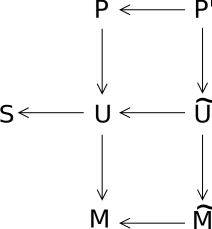
\includegraphics[width=2in]{commute.pdf}
%\end{figure}
%
%\newpage
%\subsection{The Euclidean cone surface $\mathbf{M}$}
%\compat{I would say: Observe that translations of ${\mathbb R}^2$ by pairs even integers preserves the subset ${\mathbf P}$ and respects the equivalence relation defining ${\mathbf U}$. Thus this gives an action of $(2{\mathbb Z})^2$ on ${\mathbf U}'$. We define ${\mathbf M}$ to be the quotient. It is depicted in Figure ...}
%
%Observe that the translations by pairs of even integers preserves the subset $\mathbf P$ and respects the equivalence relation on $\mathbf U$
%
%We will call this quotient space $\mathbf{M}$ and define it as such:
%\begin{Def}{$\mathbf{M}$.}\\
%$\mathbf{M}$ is a base surface of $\mathbf{U}'$ given by the quotient $\mathbf{U}'/2\mathbb{Z}\oplus2\mathbb{Z}$, where $2\mathbb{Z}\oplus2\mathbb{Z}\times\mathbf{U}'\rightarrow\mathbf{U}'$ is the group action on $\mathbf{U}'$ defined as $(m,n)\circ(u,v)=(u+m,v+n)$.
%\end{Def}
%
%\begin{figure}[H]
%\begin{center}
%\includesvg[width=2in.]{unfoldcutquotient}\hspace{0.2in}
%\includesvg[width=2in.]{quotient}
%\end{center}
%\caption{$\mathbf{U}'$ equivalence classes under group action (left), and $\mathbf{M}$ with identified edges and vertices (right).}
%\label{fig:quotient}
%\end{figure}
%
%The quotient space is a genus 1 surface that resembles a $2\times2$ torus with a unit square removed from it. Near the outer vertex it behaves as a torus might. The inner vertices $c_{1},c_{3}$ have cone angle $\frac{3\pi}{2}$, and $c_{2}$ has a cone angle of $3\pi$. None of these inner vertices have cone angles that are integral multiples of $2\pi$, so in order to create the necessary translation surfaces we require the minimal number of copies of both $\mathbf{U}$ and $\mathbf{M}$ to construct their associated phase spaces.  \compat{Move the discussion of building the translation surface to the next section. Otherwise this paragraph is good.}

\section{Proof of Main Theorem}
The following section studies the translation surface's various symmetries and associated Veech group. In doing so, we establish what sorts of properties of $\tilde{\mathbf{M}}$ remain invariant when undergoing affine transformations. Since $\tilde{\mathbf{U}}$ is a cover of $\tilde{\mathbf{M}}$, we will study the first homology classes of $\tilde{\mathbf{M}}$ that realize $\tilde{\mathbf{U}}$ as a $\mathbb{Z}^2$ cover. The goal in the end is to construct a basis for the homotopy classes of paths on $\tilde{\mathbf{M}}$ that can be lifted onto $\tilde{\mathbf{U}}$. We generalize how the Veech group of $\tilde{\mathbf{M}}$ acts on homology, and show that closed geodesics on the base surface whose lifts onto the $\mathbb{Z}^2$-cover extend to a homomorphism of $\pi_1(\tilde{\mathbf{M}})$ to $\mathbb{Z}^2$. The kernel of this homomorphism determines the cover, and any element of the Veech group acting on $\tilde{\mathbf{M}}$ will stabilize the surface and extend to an isomorphism of its homology classes.

\subsection{Veech Group and Symmetries}
Observe that $\tilde{\mathbf{M}}$ shares symmetries with the square (up to translation). This is made obvious by the fact that $\tilde{\mathbf{M}}$ is tiled by squares. Any rotations and reflections acting on $\tilde{\mathbf{M}}$ respects its boundaries. We use their matrix representations, and consider only the orientation preserving transformations of determinant one.

Theorems of Gutkin and Judge tell us that any Veech surface that is tiled by squares has a Veech group that is a finite-indexed subgroup of $SL_2(\mathbb Z)$. Therefore the group is a lattice in $SL_2(\mathbb R)$. We will call the Veech group of $\tilde{\mathbf{M}}$, $\Gamma$. $\Gamma$ will without a doubt be generated by parabolic elements, such as skew matrices, and $\tilde{\mathbf{M}}$'s various isometries. 

It is easily shown that $SO_2(\mathbb Z)\subset\Gamma$. Consider a rotation about the center of any square. By a series of cutting and gluing operations, $\tilde{\mathbf{M}}$ can be reconstruced as a staircase again, sending one edge to exactly one other.

Each square is unit, and any pair of edges have two squares between them. This gives rise to a very natural cylinder decomposition of $\tilde{\mathbf{M}}$ in both horizontal and vertical directions.



The staircase is then decomposed into 6 uniform cylinders of moduli $\frac{1}{2}$ in both the vertical and horizontal directions. Any geodesic on the horizontal cylinders are incident with exactly two other geodesics on the vertical cylinders.

\begin{Def}
The \textbf{set of horizontal cylinders} of $\tilde{\mathbf{M}}$, denoted $\Delta_{i}$ $(1\leq i \leq 6)$, are the cylinders with boundaries formed by saddle connections made between unions of singularities in the horizontal direction. \newline
Likewise, the \textbf{set of vertical cylinders}, denoted $\varepsilon_j$ $(1\leq j 
\leq 6)$, are the cylinders with boundaries formed by saddle connections made between unions of singularities in the vertical direction. \newline
Refer to Figure $\ref{fig:decomp}$ for the decomposition
\end{Def}

Horizontal and vertical cylinders of the surface are disjoint within their respective sets, and their union is the surface $\tilde{\mathbf{M}}$.

  Recall that the modulus of a cylinder, $\mu$, is given by the ratio of the cylinder's width to its circumference, $\mu{}={}w/c$. A surface that is composed entirely out of similar horizontal and vertical cylinders is stabilized by Dehn-twists whose derivatives are matrices of magnitude $\lambda$ equal to that of lowest common multiple of the inverse moduli, $\mu^{-1}$. [cite Veech 89?]



In this case, the moduli are easily obtained and uniform throughout $\tilde{\mathbf{M}}$'s cylinders. We can see that any skews of magnitude $\lambda=\pm2$, since $\mu^{-1}{}=2$, are derivatives of Dehn-twists that preserve the boundaries of the cylinders. Figure $\ref{fig:skew}$ demonstrates a Dehn-twist of magnitude 2 acting on both horizontal and vertical cylinders. Hence the derivatives, 
\begin{equation}
\left[ \hspace{1mm} \begin{matrix}
				1 & \pm 2\\
				0 & 1
			\end{matrix}\hspace{1mm}\right],\text{ and }
			\left[ \hspace{1mm} \begin{matrix}
							1 & 0\\
							\pm 2 & 1
						\end{matrix}\hspace{1mm}\right]
\end{equation}
are the parabolic generators of $\Gamma$. The fact that $\lambda=1$ does \emph{not} stabilize $\tilde{\mathbf{M}}$ is an absolutely integral part of the major proof.

\newpage
\subsection{Defining Homology Classes of $\tilde{\mathbf{M}}$}
\compav{TODO:\\
Construct homotopy class 12-gon\\
Construct staircase with class intersection\\}
The cylinder decomposition of $\tilde{\mathbf{M}}$ into 12 vertical and horizontal cylinders naturally produce a set of closed homotopic paths that travel along the cylinder's circumference. Because of $\tilde{\mathbf{M}}$'s translational symmetries, we consider every cylinder to contain a set of homologous paths, characterized by the geodesic running along the cylinder's meridian. 

Since none of these paths can't be contracted into a single point or deformed into another path without crossing over a singularity, they are non-trivial and span the set of homology classes of $\tilde{\mathbf{M}}$. We denote the set of closed paths on the cylinders by $\gamma_{0,..,11}$, where the even-indexed paths are horizontal and the odd-indexed paths are vertical. (see figure)

From these paths we create the following homology classes that determine our $\mathbb{Z}^2$-cover:



Here $u,v,$ and $z$ belong to $H_1(\tilde{\mathbf{M}},\mathbb Z)$. These classes are generalizations of differential 1-forms, say $dx,dy,dz$, on the four-fold cover whose path integrals on $\tilde{\mathbf{M}}$ map directly to the cover.  In our case, there is translational symmetry and it is understood that any geodesic with rational slope is periodic, so we need only consider $\tilde{\mathbf{M}}$'s homology classes. Let $\alpha$ be a closed path on $\tilde{\mathbf{M}}$ as an element of $\pi_1(\tilde{\mathbf{M}})$. The intersection number of any two homology classes is given as the bilinear form:

\begin{align}
i:H_1(\tilde{\mathbf{M}},\mathbb Z)\times H_1(\tilde{\mathbf{M}},\mathbb Z)\rightarrow \mathbb Z.
\end{align}

The $\mathbb{Z}^2$ cover, $\tilde{\mathbf{U}}$, is associated to the kernel of the homomorphism
\begin{align}
\Omega_{u,v}:\pi_1(\tilde{\mathbf{M}})\rightarrow \mathbb{Z}^2, \alpha\mapsto(i(u,[\alpha]),i(v,[\alpha])).
\end{align}
The classes u and v determine where the lifted geodesic terminates on $\tilde{\mathbf{U}}$. Careful experimentation and observation shows us that these classes correspond to moving along the horizontal and vertical directions relative to $\tilde{\mathbf{U}}_0$'s hole indexing convention. We suspect that the remaining z class is some remnant of how the quotient topology of $\tilde{\mathbf{U}}_0$ identifies a point on the boundary of a hole with another as an element of $\mathbb{Z}/4\mathbb Z$, as these are the cylinders of $\tilde{\mathbf{U}}_0$ that cross from one phase to the next (See Figure $\ref{fig:mtilda}$). Regardless, the classes $u,v$ are enough to determine $\tilde{\mathbf{U}}$'s fundamental group as they already take into consideration the effect that the rotations of $\tilde{\mathbf{U}}_0$ has on $\tilde{\mathbf{U}}$'s translational symmetries.
\newpage
\subsection{Horizontal, Vertical, and Slope One Cylinders of $\tilde{\mathbf{M}}$}
\begin{figure}[H]
\centering
\includesvg[pretex=\tiny, width=4in]{slopeonecylinder}
\end{figure}
\newpage
\subsection{Slope Normalization Algorithm}
\newpage
\subsection{Proof of Theorem}

\begin{figure}[H]
\includesvg[width=2.3in]{cubesxyzpaths}\hspace{0.1in}
\raisebox{0.5in}{\includesvg[width=2.2in]{unfoldcutpath}}
\\ \text{Here we can see paths a,b, and c on }$\mathbf{U}$\text{ and }$\mathbf{S}$,
\\ \text{where their initial trajectories are (0,1), (1,0), and (1,1) respectively.}
\end{figure}

\end{document}
